
% This LaTeX was auto-generated from MATLAB code.
% To make changes, update the MATLAB code and republish this document.

\documentclass{article}
\usepackage{graphicx}
\usepackage{color}
\usepackage{color,amsmath,amssymb,amsthm}
\sloppy
\definecolor{lightgray}{gray}{0.5}
\setlength{\parindent}{0pt}

\begin{document}

    
    
\section*{Reference Answers to Assignment 2 of Numerical Algorithms with Case Studies}

\begin{par}

Here are TA's reference answers, not standard answers. If you have any different ideas,
please feel free to let us know. Anyone who first finds out errors in this doc will receive
additional rewards(up to 5) for this assigment.

\end{par} \vspace{1em}

\subsection*{Contents}

\begin{itemize}
\setlength{\itemsep}{-1ex}
   \item Question 1
   \item Question 2
   \item Question 3
   \item Functions metioned in the doc.
\end{itemize}


\subsection*{Question 1}

\begin{par}

 (10 pts) Conduct Gaussian elimination on
\begin{align*}
G = \begin{bmatrix}
1&0&0&5\\
1&1&-3&-1\\
2&3&-1&1\\
-2&3&-2&0
\end{bmatrix}
\end{align*}
and find its LU decomposition.

\end{par} \vspace{1em}
\begin{par}

Answer:
\begin{align*}
G = \begin{bmatrix}1&0&0&5\\1&1&-3&-1\\2&3&-1&1\\-2&3&-2&0\end{bmatrix}
&=\begin{bmatrix}1& & &\\ &1& &\\ & &1&\\ & & &1\end{bmatrix}
\begin{bmatrix}1&0&0&5\\1&1&-3&-1\\2&3&-1&1\\-2&3&-2&0\end{bmatrix}\\
&=\begin{bmatrix}1& & &\\ 1&1& &\\ 2& &1&\\ -2& & &1\end{bmatrix}
\begin{bmatrix}1&0&0&5\\&1&-3&-6\\&3&-1&-9\\&3&-2&-10\end{bmatrix}\\
&=\begin{bmatrix}1& & &\\ 1&1& &\\ 2&3&1&\\ -2&3& &1\end{bmatrix}
\begin{bmatrix}1&0&0&5\\&1&-3&-6\\&&8&-9\\&&7&28\end{bmatrix}\\
&=\begin{bmatrix}1& & &\\ 1&1& &\\ 2&3&1&\\ -2&3&\frac{7}{8}&1\end{bmatrix}
\begin{bmatrix}1&0&0&5\\&1&-3&-6\\&&8&-9\\&&&\frac{161}{8}\end{bmatrix}\\
\end{align*}

\end{par} \vspace{1em}


\subsection*{Question 2}

\begin{par}

 (10 pts) Write your own codes for forward substitution or back substitution (choose the one
you like).  Conduct random tests to show that its computational complexity is proportional
to $n^2$(n is the size of the matrix) by making a plot.  (Hint:for each
tested n, conduct for example 10 random tests and compute the average time.)

\end{par} \vspace{1em}
\begin{par}

Answer:\\
The following function $tri\_system\_solver$ offers two algorithms to solve a triangular
system: row oriented method and column oriented method given the triangular $T$ and vector $b$ as the first
two parameters of the function. To use different algorithm, change its third parameter
$row\_oriented$ to be true or false.\\\\
If the input matrix is an upper triangular matix, the function will apply back
substitution method. If the input matrix is a lower triangular matrix, the
function will apply forward substitution method. Be sure to input a
triangular matrix, or the result may be wrong. \\\\
The two algorithms perform different in efficiency. If you noticed the
different performance of matrix multiplication in assignment 1, you will know
why column oriented method is faster immediantly.
\begin{verbatim}
function [ x ] = tri_system_solver(T, b, row_oriented)
if nargin<3
      row_oriented = true;
end
n = size(T,1);
x = zeros(n,1);
if row_oriented
    if T(1,n) == 0 %Forward Substitution for Lower Triangular System
        for i = 1:n
            x(i) = (b(i) - T(i,1:i-1)*x(1:i-1))/T(i,i);
        end
    else %Back Substitution for Upper Triangular System
        for i = n:-1:1
            x(i) = (b(i) - T(i,i +1:n)*x(i+1:n))/T(i,i);
        end
    end
else
    if T(1,n) == 0 %%Forward Substitution for lower triangular system
        index = 1:n;
    else %Back Substitution for upper triangular system
        index = n:-1:1;
    end
    for i = index
        x(i) = b(i)/T(i ,i);
        b = b - T(:, i) * x(i);
    end
end
\end{verbatim}
Function $rand\_tri$ in the codes above is for generating random triangular matrix and
listed with its details in the end of this doc.
Now check the correctness of this solver.

\end{par} \vspace{1em}
\begin{verbatim}
error = 0;
n = 200;
for i=1:1000
    T = rand_tri(n,rand>0.5); %generate lower or upper triangular system randomly
    b = rand(n,1);
    re = tri_system_solver(T, b, rand>0.5);%use the two method randomly
    loss = sum((T*re-b).^2)/sum(b.^2);
    error = max(loss,error);
end
fprintf('The relative error is %g.\n',error);
\end{verbatim}

        \color{lightgray} \begin{verbatim}The relative error is 7.25271e-28.
\end{verbatim} \color{black}
    \begin{par}

We can confirm the correctness of the solver as the relative error is smaller than machine precision.\\\\
Next I will conduct random tests to show its computational complexity.
The function $time\_test\_tri$ in the codes below is for computing the
time used with matrix dim n and given algorithm for 100 computations
and is listed with its details in the end.

\end{par} \vspace{1em}
\begin{verbatim}
ns = (1:30)*100;
times = zeros(2,30);
for i = 1:30
    times(1,i) = time_test_tri(ns(i), 1);
    times(2,i) = time_test_tri(ns(i), 0);
end
plot(ns,3.2*1e-7*ns.^2,ns,1.06*1e-7*ns.^2,ns,times(1,:),'o',ns,times(2,:),'*');
xlabel('matrix dim');
ylabel('time used');
legend('y = 3.2\times 10^{-7}x^{2}','y = 1.06\times 10^{-7}x^{2}',...
    'row oriented method','column oriented method','Location','best');
title("Triangular System Solver's Computational Complexity");
\end{verbatim}

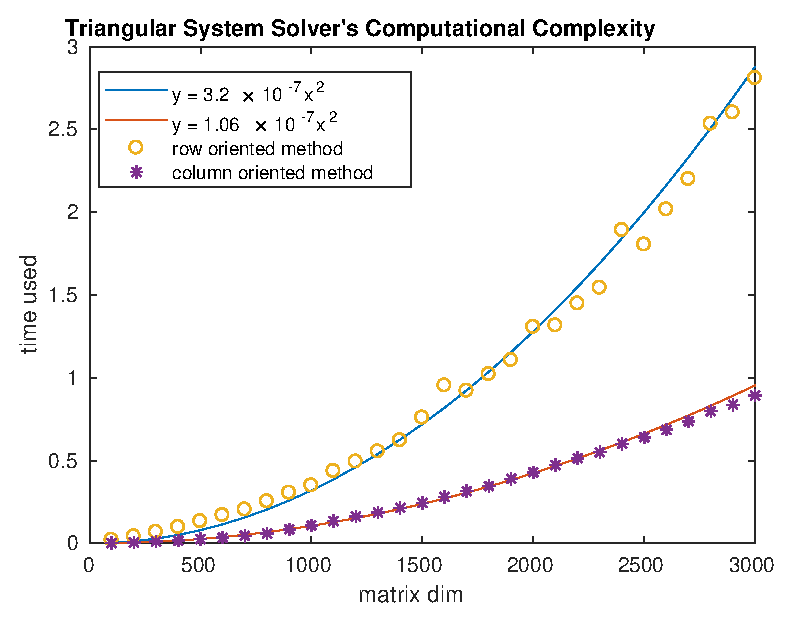
\includegraphics [width=4in]{main_01.eps}
\begin{par}

The figure shows that the complexity is $o(n^2)$ for both algorithms but
the coefficients are different.

\end{par} \vspace{1em}


\subsection*{Question 3}

\begin{par}

(20 pts) Write your own codes for the $LU$ decomposition of a matrix $A$ and test the correctness
of  your  codes  by  computing  the  error  between $A$ and $LU$,  where $L$ and $U$ are  the  lower
triangular and upper triangular matrices obtained from your codes.  Conduct random tests to
show that its computational complexity is proportional to $n^3$(n is the size of the matrix) by
making a plot.

\end{par} \vspace{1em}
\begin{par}

Answer:\\
The following two functions offer two algorithms to solve a $LU$
decomposition: row oriented and column oriented. The row oriented algorithm uses
the pseudocodes discussed in class. \\\\
The column oriented algorithm will return a
unit upper triangular matrix, which is different from the method
discussed in class. But they all return a $LU$ decompostion. It's easy for column oriented
algorithm to change itself to return a unit lower triangular matrix. If
you have no idea how to make it, feel free to contact me.\\\\
You will find the two algorithms perform different in efficiency.\\\\
Function $LU\_s$ applies the method discussed in class.
\begin{verbatim}
function [L,U] = LU_s(A)
[m,n] = size(A);
L = eye(n);
U = A;
if m~=n
    fprintf('Dim error\n');
    return
end
for k= 1:n
    for j= (k+1):n
        L(j,k) = U(j,k)/(U(k,k)+eps);
        for i = k:n
            U(j,i) = U(j,i) - L(j,k)*U(k,i);
        end
    end
end
end
\end{verbatim}
Function $LU\_f$ will be faster.
\begin{verbatim}
function [L,U] = LU_f(A)
[m,n] = size(A);
U = eye(n);  % initialize
L = A;
if m~=n
    fprintf('Dim error\n');
    return
end
for k= 1:n
    for j= (k+1):n
        U(k,j) = L(k,j)/(L(k,k)+eps);
        L(:,j) = L(:,j) - U(k,j)*L(:,k);
    end
end
end
\end{verbatim}
Now check the correctness.

\end{par} \vspace{1em}
\begin{verbatim}
error = 0;
loss = 0;
for i = 1:100
    A = rand(100) + eye(100);
    [L1,U1] = LU_f(A);
    [L2,U2] = LU_s(A);
    error = max(error, norm(L1-tril(L1),'fro'));
    error = max(error, norm(L2-tril(L2),'fro'));
    error = max(error, norm(U1-triu(U1),'fro'));
    error = max(error, norm(U2-triu(U2),'fro')); % check the triangular matrix
    loss = max(loss, norm(L1*U1-A,'fro'));
    loss = max(loss, norm(L2*U2-A,'fro')); % check the decomposition
end
fprintf('The max difference between the results and triangular matrix is %g.\n',error);
fprintf('The max decomposition loss is %g.\n',loss);
\end{verbatim}

        \color{lightgray} \begin{verbatim}The max difference between the results and triangular matrix is 9.17958e-10.
The max decomposition loss is 1.42533e-09.
\end{verbatim} \color{black}
    \begin{par}

Now I will conduct random tests to show its computational complexity.
Function $time\_test\_lu$ is for computing the time used for 100 computations
and is listed with its details in the end.

\end{par} \vspace{1em}
\begin{verbatim}
ns = (1:25)*20;
times = zeros(25,2);
for i = 1:25
    times(i,:) = time_test_lu(ns(i));
end
plot(ns,2.535*1e-7*ns.^3,ns,5.02*1e-8*ns.^3,ns,times(:,1)','o',ns,times(:,2)','*');
xlabel('matrix dim');
ylabel('time used for 100 computations');
legend('y=2.535\times 10^{-7}x^3','y=5.02\times 10^{-8}x^3',...
    'method using pseudocodes in class','column oritend method','Location','best');
title("LU decomposition's computation complexity");
\end{verbatim}

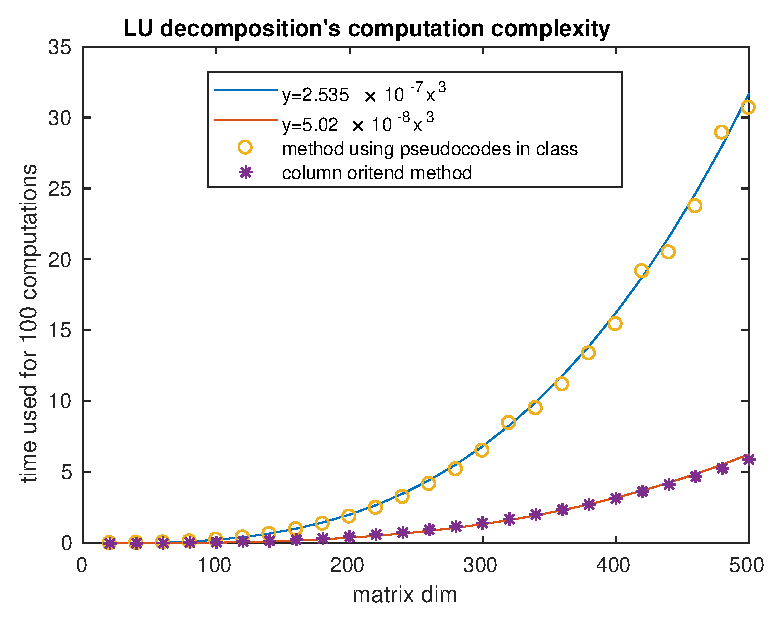
\includegraphics [width=4in]{main_02.eps}


\subsection*{Functions metioned in the doc.}

\begin{par}

Function $rand\_tri$ is for generating random triangular matrix in Question 2.
\begin{verbatim}
function [ T ] = rand_tri( n , islower )
T = ones(n);
for i=1:n
    T(i+1:n,i) = 0;
end
if islower
    T = T';
end
T = T.*rand(n)+eye(n);% make sure T is well-conditioned.
end
\end{verbatim}
Funtion $time\_test\_tri$ is for computing the time used with 100
computations for triangular system solver in
Question 2.
\begin{verbatim}
function [ t ] = time_test_tri(n, row_oriented)
T = rand_tri(n,0);
b = rand(n,1);
tic;
for i=1:500
    tri_system_solver(T,b,row_oriented);
end
t = toc;
end
\end{verbatim}
Function $time\_test\_lu$ is for computing the time used with 100 computations
for LU decomposition in Question 3.
\begin{verbatim}
function [ t ] = time_test_lu(n)
A = rand(n);
A = A*A';
t = [0 0];
tic;
for i=1:200
    LU_s(A);
end
t(1) = toc;
tic;
for i=1:200
    LU_f(A);
end
t(2) = toc;
end
\end{verbatim}

\end{par} \vspace{1em}



\end{document}
    
